\documentclass[12pt,oneside, a4paper]{book}
\usepackage[utf8]{inputenc}
\usepackage[croatian]{babel}
\usepackage[margin=1in]{geometry}
\usepackage{multirow}

\usepackage{listings}
\usepackage{xcolor}
\usepackage{chngcntr} % Paket za manipulaciju brojačima

\counterwithout{section}{chapter} % Odvaja sekcije od poglavlja
\renewcommand{\thesection}{\arabic{section}} % Postavlja format numeracije na 1, 2, 3...

\lstdefinestyle{bashstyle}{
     backgroundcolor=\color{gray!10},
     basicstyle=\ttfamily\small,
     keywordstyle=\bfseries,
     frame=single,
     rulecolor=\color{gray!50},
     breaklines=true,
     showstringspaces=false,
     morekeywords={source, export, sudo, roscore, rosrun, roslaunch}
}

\lstdefinestyle{cppstyle}{
     backgroundcolor=\color{gray!5},
     basicstyle=\ttfamily\small,
     keywordstyle=\color{blue}\bfseries,
     commentstyle=\color{gray},
     stringstyle=\color{red},
     frame=single,
     rulecolor=\color{gray!50},
     breaklines=true,
     showstringspaces=false,
     language=C++
}

\usepackage{textcomp}
\usepackage{gensymb}
\usepackage{bigstrut}
\usepackage{amsmath}
\usepackage{amsfonts}
\usepackage{amssymb}
\usepackage[hidelinks]{hyperref}
\usepackage{enumitem}
\usepackage{lmodern}
\usepackage{datetime}
\usepackage{pgfplots}
\usepackage{tikz}
\usepackage{float}
\usepackage{fancyhdr} 
\usepackage{titlesec} 
\pgfplotsset{compat=1.16}
\usepackage{makecell}
\usepackage{nomencl}
\usepackage[table,xcdraw]{xcolor}
\usepackage{graphicx} 

% Podesavanje izgleda referenci
\usepackage[square, numbers, sort]{natbib} 
\addto\captionscroatian{%
  \renewcommand{\bibname}{Literatura}
}

% Podešavanje izgleda naslova sekcije (da izgleda moćno, ali bez nove stranice)
\titleformat{\section}[hang]
  {\normalfont\huge\bfseries}{\thesection}{1em}{}
\titlespacing*{\section}{0pt}{3.5ex plus 1ex minus .2ex}{2.3ex plus .2ex}

% Podešavanje zaglavlja i podnožja (Header & Footer)
\renewcommand{\footrulewidth}{0.4pt}
\renewcommand{\sectionmark}[1]{\markboth{#1}{}} % Koristimo sectionmark umjesto chaptermark
\renewcommand{\headrulewidth}{0.4pt}
\addtolength{\headheight}{15pt}

\fancypagestyle{fancyplain}{%
  \fancyhf{}
  \lhead{\nouppercase{\fancyplain{}{\leftmark}}} % Dinamički ispisuje naziv trenutne \section u zaglavlju
  \renewcommand{\footrulewidth}{0.4pt}
  \lfoot{\slshape Klisura I., ”AGC (Automatic Generation Control)”}
  \rfoot{\thepage}
  \cfoot{}
}

% Za prve strane sekcija (gdje ne želimo liniju na vrhu)
\fancypagestyle{plain}{%
  \fancyhf{}
  \lfoot{\slshape Klisura I., ”AGC (Automatic Generation Control)”}
  \rfoot{\thepage}
  \renewcommand{\headrulewidth}{0pt}
}

% Iskljucivanje broja strane iz Sadrzaja, Popisa slika i Popisa tabela
\AtBeginDocument{\addtocontents{toc}{\protect\thispagestyle{empty}}}
\AtBeginDocument{\addtocontents{lof}{\protect\thispagestyle{empty}}}
\AtBeginDocument{\addtocontents{lot}{\protect\thispagestyle{empty}}}

% Nazivi u "Literatura", "Tabela"...
\addto\captionscroatian{%
  \renewcommand{\bibname}{Literatura}
  \renewcommand{\tablename}{Tabela}
  \renewcommand{\nomname}{Popis oznaka}
  \renewcommand{\indexname}{Indeks pojmova}
  \renewcommand{\lstlistingname}{Program}
}
\addto\captionscroatian{\renewcommand{\listtablename}{Popis tabela}}

\begin{document}
\begin{titlepage}
\begin{center}


\includegraphics[width=0.25\textwidth]{logo_etf.png}~\\[0.1cm]
\textsc{\Large Univerzitet u Sarajevu}\\[0.2cm]  
\textsc{\Large Elektrotehnički fakultet}\\[0.2cm] 
\textsc{\Large Odsjek za automatiku i elektroniku}\\[0.2cm]
\textsc{\Large Strukture i režimi rada elektroenergetskih sistema}\\[0.2cm]
\textsc{\large Akademska 2025/26. godina}\\[3cm]
\hrule
\vspace{0.5cm}
{\huge \bfseries AGC (Automatic Generation Control)} \\[0.4cm] 
\hrule 
\vspace{0.5cm}

\textsc{\Large Seminarski rad}\\
\textsubscript{}\\[5cm]

% Autor
\textbf{\Large Studentica:\\ \Large Ismihana Klisura\\ [0.2cm]}
\vfill

% Dno stranice  
{\large Sarajevo, juli 2026.}

\end{center} 
\end{titlepage}

\frontmatter
\pagenumbering{arabic} % PRISILJAVA ARAPSKE BROJEVE (1, 2, 3) OD SAMOG POČETKA
\pagebreak

\section*{Sažetak}

U radu je predstavljen razvoj dinamičkog konvertora koji statičke podatke
elektroenergetske mreže automatski pretvara u
dinamičke modele sa AGC (\emph{Automatic Generation Control}) regulacijom
frekvencije, pogodne za vremensku simulaciju u dTwin okruženju. Konvertor je
realizovan u C++ kao plugin (dinamička biblioteka) sa grafičkim interfejsom
u natID biblioteci. Kroz XML konfiguracijski fajl korisnik navodi brojeve
generatora koji dobijaju AGC model (primarna droop regulacija, sekundarna
integralna regulacija, turbinski governor i limiter snage), dok svi ostali
generatori dobijaju standardni model bez regulacije. Konverzija se izvršava
u zasebnom threadu uz indikator napretka u drugom threadu, a admitansna
matrica mreže realizovana je natID dense matricama. Numerička robusnost
postignuta je inicijalizacijskim podmodelom koji rješava tokove snaga i
dinamičku simulaciju pokreće iz tačne ravnotežne tačke. Ispravnost rješenja
demonstrirana je simulacijom skoka opterećenja: na sistemima Case~9, Case~30
i Case~118 frekvencija se nakon propada i prigušenih oscilacija vraća tačno
na nominalnih 50~Hz, čime je potvrđeno ispravno djelovanje sekundarne
regulacije. Za Case~300 konverzija je uspješna, a simulacija je
identifikovana kao ograničenje klasičnog modela generatora u mrežama sa
ekstremnim naponskim profilom.

\vspace{0.3cm}
\noindent\textbf{Ključne riječi:} AGC, sekundarna regulacija frekvencije,
droop regulacija, dinamički konvertor, MATPOWER, dTwin, natID, C++ plugin,
tokovi snaga, sinhroni generator

\vspace{0.8cm}

\section*{Abstract}

This paper presents the development of a dynamic converter that
automatically transforms static power system data 
into dynamic models with AGC (Automatic Generation Control) frequency
regulation, suitable for time-domain simulation in the dTwin environment.
The converter is implemented in C++ as a plugin (dynamic library) with a
graphical user interface built on the natID library. Through an XML
configuration file, the user specifies the numbers of generators that
receive the AGC model (primary droop control, secondary integral control,
turbine governor, and power limiter), while all remaining generators receive
a standard model without regulation. The conversion runs in a separate
thread with a real-time progress indicator in a second thread, and the
network admittance matrix is built using natID dense matrices. Numerical
robustness is achieved through an initialization submodel that solves the
power flow problem and starts the dynamic simulation from an exact
equilibrium point. The correctness of the solution is demonstrated by
simulating a load step: on Case~9, Case~30, and Case~118, the system
frequency, after a dip and damped oscillations, returns exactly to the
nominal 50~Hz, confirming the correct operation of secondary frequency
control. For Case~300, the conversion completes successfully, while the
simulation is identified as a limitation of the classical generator model
in networks with an extreme voltage profile.

\vspace{0.3cm}
\noindent\textbf{Keywords:} AGC, secondary frequency control, droop control,
dynamic converter, MATPOWER, dTwin, natID, C++ plugin, power flow, synchronous generator

%\newpage

\tableofcontents
\listoffigures
\addcontentsline{toc}{chapter}{Popis slika}

\newpage 
\cleardoublepage % start new page
\pagestyle{fancyplain} % puts headers/footers back on


%\mainmatter
\section{Opis projekta}
 
Stabilnost frekvencije jedan je od temeljnih zahtjeva pouzdanog rada
elektroenergetskog sistema. Frekvencija sistema direktno odražava balans
između proizvedene i potrošene aktivne snage: svaki višak potrošnje usporava
rotore sinhronih generatora i obara frekvenciju, dok višak proizvodnje
frekvenciju podiže. Kako se opterećenje mreže neprestano mijenja, potreban je
automatski mehanizam koji proizvodnju kontinuirano prilagođava potrošnji i
frekvenciju drži na nominalnoj vrijednosti od 50~Hz.
 
Taj mehanizam ostvaruje se kroz dva hijerarhijska nivoa regulacije. Primarna
regulacija (statizam, engl. \emph{droop}) je brza, proporcionalna reakcija
turbinskih regulatora na odstupanje brzine rotora -- ona zaustavlja propad
frekvencije, ali po svojoj prirodi ostavlja trajno odstupanje od nominalne
vrijednosti. Sekundarna regulacija, poznata kao AGC (\emph{Automatic
Generation Control}), integralnim djelovanjem pomjera referentnu snagu
odabranih agregata sve dok se frekvencija ne vrati tačno na nominalnu
vrijednost. AGC tematika obrađena je u ovom projektu.\\
 \newline
Cilj projekta je razvoj dinamičkog konvertora koji statičke podatke
elektroenergetske mreže (MATPOWER testni slučajevi \texttt{case9},
\texttt{case30}, \texttt{case118} i \texttt{case300}) automatski pretvara u
dinamički model pogodan za vremensku simulaciju u dTwin okruženju. Konvertor je projektovan tako da, prema zahtjevima teme, ispunjava sljedeće stavke:
\begin{itemize}
  \item realizovan je u C++ kao plugin u formi dinamičke biblioteke (dll) koju dTwin učitava,
  \item posjeduje grafički korisnički interfejs razvijen u natID biblioteci,
  \item kroz XML konfiguracijski fajl korisnik navodi brojeve generatora koji dobijaju AGC model regulacije, dok svi ostali generatori dobijaju standardni model bez regulacije,
  \item konverzija se izvršava u zasebnom threadu, dok drugi thread u realnom vremenu prati napredak konverzije,
  \item sve matrice (admitansna matrica mreže) realizovane su korištenjem natID dense matrica,
  \item konvertor je testiran na sva četiri zadana testna slučaja.
\end{itemize}
 
% [OVDJE UBACI OpenDraw DIJAGRAM ARHITEKTURE - blok šema toka podataka]
\begin{figure}[H]
  \centering
  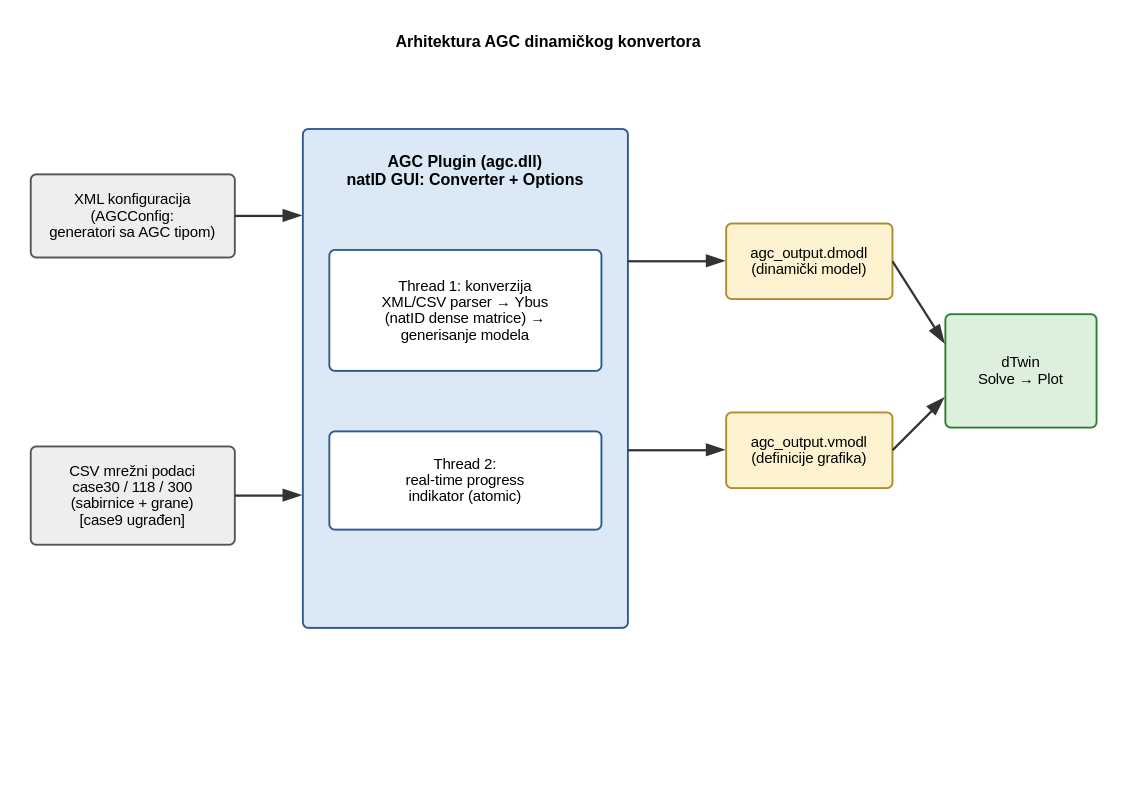
\includegraphics[width=0.9\textwidth]{arhitektura.png}
    \label{fig:arhitektura}
    \caption{Arhitektura AGC dinamičkog konvertora}
\end{figure}

\noindent Na slici~\ref{fig:arhitektura} prikazan je tok podataka kroz konvertor.
Ulaze čine dva izvora: XML konfiguracijski fajl, kojim korisnik po broju
sabirnice navodi generatore koji dobijaju AGC model regulacije (svi
nenavedeni dobijaju standardni model), i CSV fajlovi sa statičkim mrežnim
podacima -- sabirnicama (tip, opterećenje $P_L$, $Q_L$ u MW/MVAr,
proizvodnja $P_g$ u MW, zadani napon $V^{sp}$ u p.u.) i granama (otpor $R$,
reaktansa $X$ i šant susceptansa $B^{sh}$ u p.u.); podaci mreže case9
ugrađeni su direktno u konvertor. Centralni blok je AGC plugin
(\texttt{agc.dll}) sa natID grafičkim interfejsom, unutar kojeg se obrada
odvija u dvije niti: nit~1 izvršava kompletnu konverziju (parsiranje ulaza,
formiranje $Y_{bus}$ matrice natID dense strukturama, generisanje jednačina
modela), dok nit~2 u realnom vremenu prati napredak konverzije preko
atomarnog brojača. Izlaz konverzije su dva fajla: \texttt{.dmodl} sa
kompletnim dinamičkim DAE modelom (varijable, parametri, inicijalizacijski
podmodel, diferencijalne i algebarske jednačine) i \texttt{.vmodl} sa
definicijama grafika. Oba fajla preuzima dTwin, koji model rješava
(\emph{Solve}) i rezultate prikazuje (\emph{Plot}).

\begin{table}[H]
\centering
\caption{Elementi arhitekture konvertora}
\begin{tabular}{|l|l|l|}
\hline
\textbf{Element} & \textbf{Uloga} & \textbf{Format / veličine} \\ \hline
XML konfiguracija & izbor AGC generatora po broju & \texttt{id}, \texttt{type} (0/1) \\ \hline
CSV podaci & statički podaci mreže & $P_L, Q_L, P_g$ [MW], $V^{sp}$ [p.u.], $R, X, B^{sh}$ [p.u.] \\ \hline
Thread 1 & konverzija (parser, $Y_{bus}$, model) & $Y_{bus} = G + jB$ [p.u.], $S_b = 100$ MVA \\ \hline
Thread 2 & indikator napretka & progres 0--100 \% \\ \hline
\texttt{.dmodl} & dinamički DAE model & ODE + NLE jednačine \\ \hline
\texttt{.vmodl} & definicije grafika & $f$ [Hz], $\delta$ [rad], $P_m$ [p.u.] \\ \hline
dTwin & solver i vizualizacija & RK2, $\Delta t = 1$ ms \\ \hline
\end{tabular}
\end{table}
% ============ 2. MATEMATIČKI MODEL ============
\section{Matematički model}
 
\subsection{Klasični model sinhronog generatora}
 
Svaki generator predstavljen je klasičnim modelom: konstantna elektromotorna
sila $E'$ iza tranzijentne reaktanse $X_d'$. Dinamiku rotora opisuje jednačina njihanja (engl. \emph{swing} equation):
\begin{align}
  \frac{d\delta}{dt} &= (\omega - 1)\,\omega_s \label{eq:swing_delta} \\[5pt]
  \frac{d\omega}{dt} &= \frac{\omega_s}{2H}\Big(P_m - P_e - D\,(\omega - 1)\Big) \label{eq:swing_omega}
\end{align}
gdje su:
\begin{itemize}[label={}, leftmargin=1em, itemsep=0pt]
  \item $\delta$ -- ugao rotora [rad],
  \item $\omega$ -- relativna brzina rotora [p.u.],
  \item $\omega_s = 2\pi f_0$ -- sinhronska kružna frekvencija [rad/s],
  \item $H$ -- konstanta inercije [s],
  \item $D$ -- koeficijent prigušenja [p.u.],
  \item $P_m$ -- mehanička snaga [p.u.],
  \item $P_e$ -- električna snaga [p.u.].
\end{itemize}

\noindent Električna snaga koju mašina predaje mreži, u polarnim koordinatama napona sabirnice $V\angle\theta$, iznosi:
\begin{equation}
  P_e = \frac{E' V}{X_d'} \sin(\delta - \theta)
  \label{eq:pe}
\end{equation}
 
\subsection{Primarna i sekundarna (AGC) regulacija frekvencije}
 
Generatori označeni u XML konfiguraciji kao AGC tip dobijaju model turbinskog
regulatora sa primarnom i sekundarnom petljom:
\begin{align}
  \frac{dx_I}{dt} &= K_i\,(1 - \omega) \label{eq:integrator}\\[2pt]
  \frac{dP_m}{dt} &= \frac{1}{T_{gov}}\Big(P_{ref} + K_p (1-\omega) + x_I - P_m\Big)
  \label{eq:governor}\\[2pt]
  P_m^{lim} &= \mathrm{lim}\big(P_m,\, P_{min},\, P_{max}\big) \label{eq:limiter}
\end{align}
Član $K_p(1-\omega)$ predstavlja primarnu (droop) regulaciju sa statizmom
$R = 1/K_p$; integrator $x_I$ (jednačina~\ref{eq:integrator}) je sekundarna
regulacija koja eliminiše trajno odstupanje frekvencije; $T_{gov}$ je
vremenska konstanta turbine/governora, a limiter (jednačina~\ref{eq:limiter})
modeluje fizička ograničenja snage agregata. U jednačini njihanja AGC generatora umjesto $P_m$ figuriše ograničena vrijednost $P_m^{lim}$.

\begin{figure}[H]
  \centering
  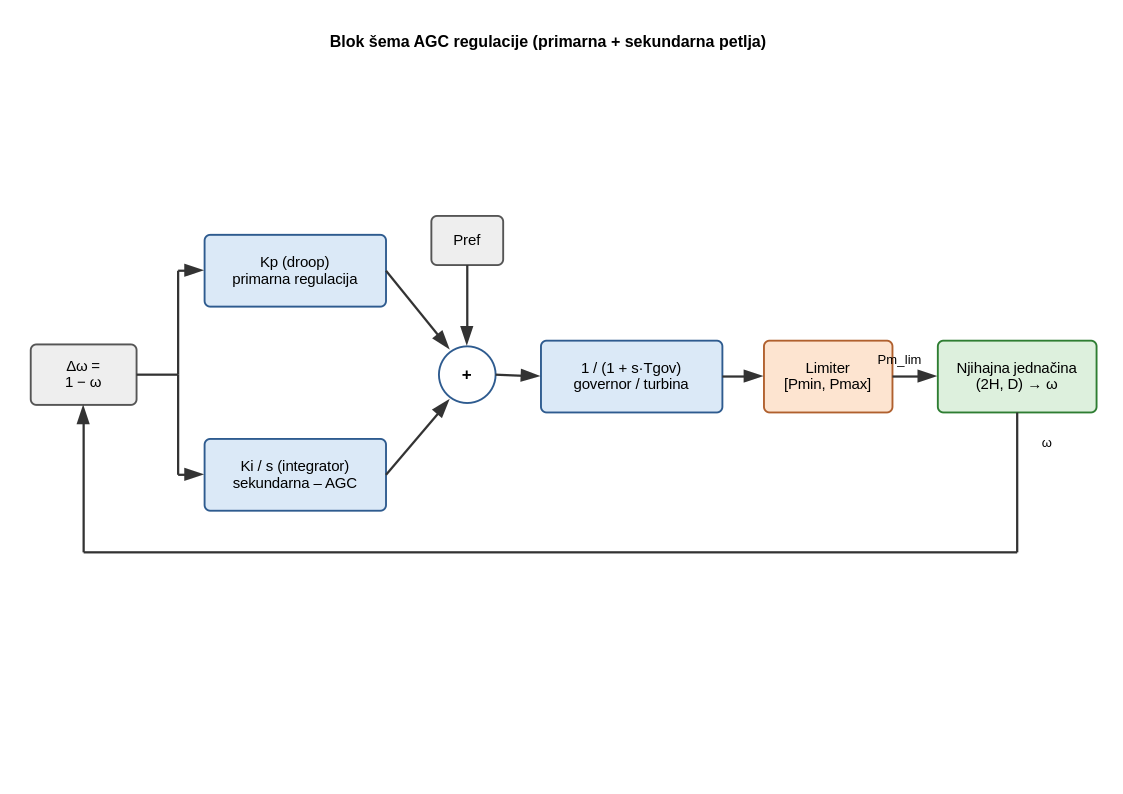
\includegraphics[width=0.8 \textwidth]{agc_blok.png}
    \caption{Blok šema AGC regulacije jednog generatora: paralelno djelovanje
  primarne (droop) i sekundarne (integralne) petlje, dinamika governora sa
  limiterom snage i povratna sprega preko jednačine njihanja}
  \label{fig:agcblok}
\end{figure}

\noindent Slika~\ref{fig:agcblok} prikazuje regulacionu petlju AGC generatora,
direktno odgovarajuću jednačinama~\ref{eq:integrator}--\ref{eq:limiter}.
Ulazni signal je odstupanje brzine rotora $\Delta\omega = 1 - \omega$
[p.u.]; pri padu frekvencije ($\omega < 1$) signal je pozitivan i regulacija
povećava snagu. Signal se paralelno vodi u dvije grane: proporcionalnu
granu $K_p$ (primarna, droop regulacija sa statizmom $R = 1/K_p$;
u projektu $K_p = 20$, tj.\ $R = 5\,\%$), koja reaguje trenutno ali ostavlja
trajno odstupanje, i integralnu granu $K_i/s$ (sekundarna regulacija, AGC;
$K_i = 5$), koja akumulira grešku frekvencije i eliminiše trajno odstupanje.
Obje grane se u sumatoru sabiraju sa referentnom snagom $P_{ref}$ [p.u.]
(radna tačka iz tokova snaga), a rezultat prolazi kroz dinamiku governora i
turbine, modelovanu prenosnom funkcijom prvog reda $1/(1+sT_{gov})$ sa
vremenskom konstantom $T_{gov} = 0{,}5$~s. Limiter ograničava mehaničku
snagu na fizički opseg agregata $[P_{min}, P_{max}]$ [p.u.]. Ograničena
snaga $P_m^{lim}$ ulazi u njihajnu jednačinu (parametri: inercija
$H = 5$~s, prigušenje $D$), čiji je izlaz brzina rotora $\omega$ --
zatvarajući povratnu spregu na ulaz. U stacionarnom stanju integrator
namješta $x_I$ tačno toliko da bude $\omega = 1$, tj.\ $f = 50$~Hz, što je
suština sekundarne regulacije.

\begin{table}[H]
\centering
\caption{Signali i blokovi AGC regulacione petlje}
\begin{tabular}{|l|l|l|l|}
\hline
\textbf{Signal/blok} & \textbf{Značenje} & \textbf{Jedinica} & \textbf{Vrijednost} \\ \hline
$\Delta\omega = 1-\omega$ & odstupanje brzine rotora & p.u. & ulaz \\ \hline
$K_p$ & droop pojačanje (primarna), $R = 1/K_p$ & -- & 20 ($R=5\,\%$) \\ \hline
$K_i/s$ & integrator (sekundarna, AGC) & 1/s & $K_i = 5$ \\ \hline
$P_{ref}$ & referentna snaga (iz tokova snaga) & p.u. & $= P_g$ \\ \hline
$1/(1+sT_{gov})$ & governor/turbina, 1.\ red & -- & $T_{gov} = 0{,}5$ s \\ \hline
$[P_{min}, P_{max}]$ & granice snage agregata & p.u. & $[0,\ 3]$ \\ \hline
$P_m^{lim}$ & ograničena mehanička snaga & p.u. & izlaz regulatora \\ \hline
$2H$, $D$ & inercija i prigušenje (njihajna jed.) & s, -- & $H=5$, $D=0{,}5$--$2$ \\ \hline
$\omega$ & brzina rotora ($f = f_0\,\omega$) & p.u. & povratna sprega \\ \hline
\end{tabular}
\end{table}

 
\textbf{Standardni generatori} (svi koji nisu navedeni u XML-u) nemaju
regulaciju: njihova mehanička snaga je konstantan parametar $P_m = P_{ref}$,
pa na poremećaj reaguju samo inercijom i prigušenjem.
 
\subsection{Mrežne jednačine}
 
Mreža je opisana admitansnom matricom $Y_{bus} = G + jB$ koja se formira iz
podataka o granama:
\begin{equation}
  Y_{ij} = -\frac{1}{R_{ij} + jX_{ij}} = G_{ij} + jB_{ij}, \quad i \neq j,
  \qquad
  Y_{ii} = \sum_{j \in \mathcal{N}(i)} \left( \frac{1}{R_{ij} + jX_{ij}} + j\frac{B^{sh}_{ij}}{2} \right)
  \label{eq:ybus}
\end{equation}
Bilansi aktivne i reaktivne snage na svakoj sabirnici $k$ (osim referentne)
formulisani su u polarnim koordinatama:
\begin{align}
  V_k \sum_m V_m \big( G_{km}\cos\theta_{km} + B_{km}\sin\theta_{km} \big) &= P_k^{inj}
  \label{eq:pbalance}\\
  V_k \sum_m V_m \big( G_{km}\sin\theta_{km} - B_{km}\cos\theta_{km} \big) &= Q_k^{inj},
  \qquad \theta_{km} = \theta_k - \theta_m
  \label{eq:qbalance}
\end{align}
Na generatorskim sabirnicama injekcija uključuje snagu mašine
(jednačina~\ref{eq:pe} i odgovarajući izraz za $Q_e$), umanjenu za lokalno
opterećenje; na potrošačkim sabirnicama injekcija je jednaka negativnom
opterećenju. Referentna (slack) sabirnica ima fiksan napon i ugao te
predstavlja beskonačnu sabirnicu.
 
\subsection{Inicijalizacija dinamičkog modela}
 
Dinamička simulacija mora krenuti iz ravnotežne tačke jer u suprotnom neuravnoteženi početni uslovi generišu vještački poremećaj koji može odvesti sistem u numeričku divergenciju. Zbog toga generisani model sadrži
inicijalizacijski podmodel (\texttt{SubModel} tipa NL) koji se rješava prije
glavne DAE simulacije:
\begin{enumerate}
  \item rješavaju se tokovi snaga mreže (jednačine~\ref{eq:pbalance}
        i~\ref{eq:qbalance}, uz $V_k = V_k^{sp}$ na PV sabirnicama),
  \item iz rješenja tokova snaga računaju se tačni početni uslovi svake
        mašine:
        \begin{equation}
          \bar{I} = \left( \frac{P + jQ}{\bar{V}} \right)^{\!*},
          \qquad
          \bar{E}' = \bar{V} + jX_d'\,\bar{I},
          \qquad
          \delta_0 = \angle \bar{E}', \quad E' = |\bar{E}'|
          \label{eq:init}
        \end{equation}
  \item početne vrijednosti se prenose u glavni model
        (\texttt{@main.} mehanizmom dTwin jezika), uz $\omega_0 = 1$,
        $P_{m,0} = P_{ref} = P_g$ i $x_{I,0} = 0$.
\end{enumerate}
Reaktivna snaga mašine pri inicijalizaciji ograničava se odozdo na
$Q \geq 0{,}1\,P_g$ (limiter minimalne pobude, engl. \emph{under-excitation
limiter}), čime se sprječava inicijalizacija mašine u podpobuđenom režimu na
granici statičke stabilnosti.
 
\subsection{Preračun reaktanse na sistemsku bazu}
 
Tranzijentna reaktansa $X_d'$ zadaje se na mašinskoj bazi, a preračunava na
sistemsku bazu $S_b = 100$~MVA:
\begin{equation}
  X_d'^{(sys)} = \frac{X_d'}{\max(1,\,P_g)}
  \label{eq:xdp}
\end{equation}
Veće mašine time dobijaju srazmjerno manju reaktansu u sistemskim p.u.
jedinicama. Bez ovog preračuna veliki agregati u \texttt{case118} i
\texttt{case300} (do 1973~MW) ne bi mogli raditi unutar granice statičke
stabilnosti ($\delta - \theta < 90^\circ$).
 
% ============ 3. IMPLEMENTACIJA ============
\section{Implementacija}
 
\subsection{Arhitektura plugina}
 
Implementacija je realizirana kao C++ plugin (dinamička biblioteka
\texttt{agc.dll}) za dTwin okruženje, korištenjem natID SDK. Plugin
implementira \texttt{sc::IPlugin} interfejs i izvozi C funkciju
\texttt{getPluginInterface()} preko koje ga dTwin učitava iz foldera
\texttt{res/plugins} i prikazuje u meniju \texttt{Model $\rightarrow$ Import}
pod imenom \emph{AGC Dynamic Converter}. Glavne komponente su:
 
\begin{itemize}
  \item \texttt{AGCPlugin.cpp/.h} -- logika konverzije: čitanje XML
        konfiguracije i CSV mrežnih podataka, sastavljanje Ybus matrice,
        generisanje \texttt{.dmodl} (dinamički model) i \texttt{.vmodl}
        (definicija grafika) fajlova, višenitno izvršavanje;
  \item \texttt{ViewConv.h} -- GUI tab \emph{Converter}: odabir ulaznog XML
        fajla, izlazne lokacije, pokretanje konverzije i statusna linija;
  \item \texttt{ViewOptions.h} -- GUI tab \emph{Options}: parametri
        simulacije (broj test slučaja, $\Delta t$, trajanje, max.\ broj
        iteracija) i parametri regulacije ($K_p$, $K_i$, $T_{gov}$,
        $P_{min}$, $P_{max}$, $H$, $D$, $X_d'$);
  \item \texttt{TabView.h}, \texttt{WindowPlugin.h} -- organizacija prozora
        i tabova (standardna natID struktura).
\end{itemize}
 
Projekat se gradi CMake sistemom (\texttt{CMakeLists.txt},
\texttt{AGCPlugin.cmake}) koji povezuje izvorni kod sa natID bibliotekama.
 
% [SLIKE GUI-ja]

\begin{figure}[H]
    \centering
    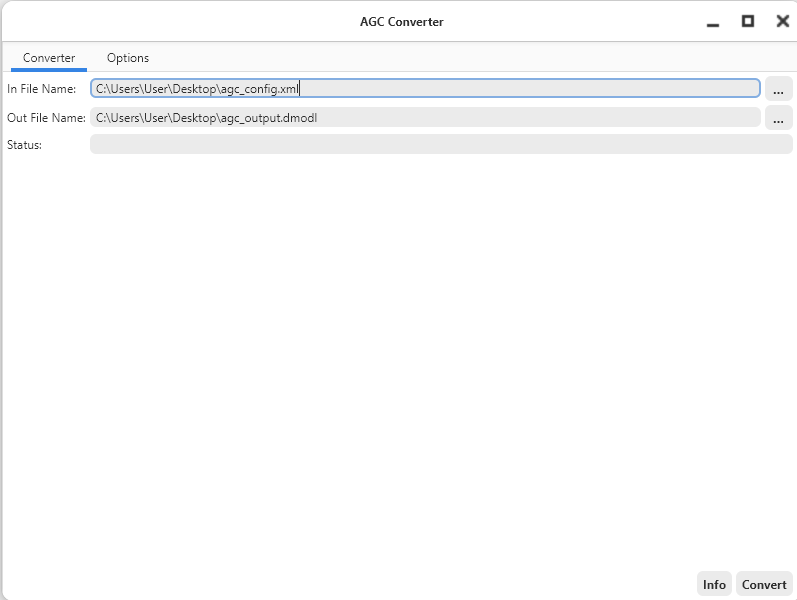
\includegraphics[width=0.8\textwidth]{konverter.png}
    \caption{Prikaz GUI-a}
    \label{fig:moj_izbor_oznake}
\end{figure}


\begin{figure}[H]
    \centering
    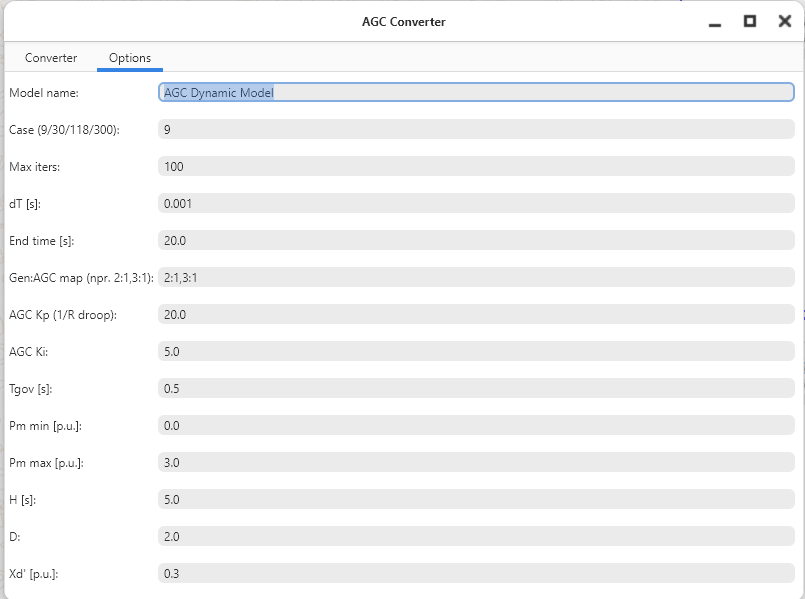
\includegraphics[width=0.8\textwidth]{options.png}
    \caption{Prikaz Options taba}
    \label{fig:moj_izbor_oznake}
\end{figure}
 
\subsection{XML konfiguracija generatora}
 
Ulazni XML fajl definiše koji generatori (po broju sabirnice) dobijaju AGC
model; svi nenavedeni generatori dobijaju standardni model, u skladu sa
specifikacijom teme. Parsiranje je realizovano natID
\texttt{xml::FileParser} (DOM) parserom.
 
\begin{lstlisting}[language=XML, style=cppstyle, caption={XML konfiguracija: generatori 2 i 22 dobijaju AGC model, ostali standardni}]
<AGCConfig>
    <Generator id="2" type="1"/>
    <Generator id="22" type="1"/>
</AGCConfig>
\end{lstlisting}
 
\subsection{Ybus matrica -- korištenje natID dense matrica}
 
U skladu sa zahtjevom teme, admitansna matrica mreže sastavljena je
korištenjem natID \texttt{dense::DblMatrix} strukture (realni dio $G$ i
imaginarni dio $B$ kao dvije matrice), prema jednačini~\ref{eq:ybus}:
 
\begin{lstlisting}[language=C++, style=cppstyle, caption={Sastavljanje Ybus matrice korištenjem natID dense::DblMatrix}]
struct YbusMatrices {
    dense::DblMatrix mG;   // realni dio admitansne matrice
    dense::DblMatrix mB;   // imaginarni dio admitansne matrice
};
 
static void buildYbus(YbusMatrices& ybus, int nBus,
                      const LineData* lines, int nLines)
{
    ybus.mG.reserve(nBus, nBus, nullptr, true);
    ybus.mB.reserve(nBus, nBus, nullptr, true);
    auto matG = ybus.mG.getManipulator1();
    auto matB = ybus.mB.getManipulator1();
    // ... nuliranje ...
    for (int l = 0; l < nLines; ++l) {
        double denom = lines[l].r*lines[l].r + lines[l].x*lines[l].x;
        double g =  lines[l].r / denom;
        double b = -lines[l].x / denom;
        matG(f, t) -= g;   matG(t, f) -= g;
        matB(f, t) -= b;   matB(t, f) -= b;
        matG(f, f) += g;   matG(t, t) += g;
        matB(f, f) += b + lines[l].b / 2.0;
        matB(t, t) += b + lines[l].b / 2.0;
    }
}
\end{lstlisting}
 
Pri generisanju mrežnih jednačina u izlaznom modelu ispisuju se samo elementi
matrice različiti od nule, čime je iskorištena rijetkost (engl.
\emph{sparsity}) strukture mreže.
 
\subsection{Višenitna konverzija sa indikatorom napretka}
 
Prema zahtjevu teme, konverzija se izvršava u zasebnom threadu (thread~1),
dok drugi thread (thread~2) u realnom vremenu prati napredak konverzije preko
atomarnog brojača koji konverzija ažurira po fazama: učitavanje podataka
(5--25\%), formiranje Ybus matrice (25--35\%), generisanje modela
(35--85\%), generisanje grafika (85--100\%).
 
\begin{lstlisting}[language=C++, style=cppstyle, caption={Višenitna organizacija konverzije}]
std::atomic<int>  progress(0);
std::atomic<bool> done(false);
 
// thread 2: real-time pracenje progresa konverzije
std::thread progressThread([&progress, &done]() {
    while (!done.load())
        std::this_thread::sleep_for(std::chrono::milliseconds(50));
});
 
// thread 1: konverzija (parsiranje, Ybus, generisanje modela)
std::thread convThread([&]() {
    progress = 5;
    // ... ucitavanje podataka, Ybus, generisanje .dmodl i .vmodl ...
    progress = 100;
    done = true;
});
 
convThread.join();
progressThread.join();
\end{lstlisting}
 
\subsection{Testni podaci}
 
Podaci \texttt{case9} mreže ugrađeni su u konvertor, dok se \texttt{case30},
\texttt{case118} i \texttt{case300} učitavaju iz CSV fajlova (sabirnice i
grane) generisanih iz originalnih MATPOWER fajlova. Snage u CSV fajlovima su
u MW i pri učitavanju se konvertuju u p.u.\ ($S_b = 100$~MVA). Za
\texttt{case300} izvršena je renumeracija sabirnica na kontinuirani opseg
1--300 (originalna MATPOWER numeracija je nekontinuirana). Generatorima se
smatraju PV sabirnice sa aktivnom proizvodnjom; sinhroni kompenzatori
($P_g = 0$) tretirani su kao PQ sabirnice. Konvertor automatski prepoznaje
referentnu sabirnicu (tip~3) -- npr.\ u \texttt{case118} to je sabirnica~69,
a ne sabirnica~1.
 
\subsection{Struktura generisanog modela}
 
Generisani \texttt{.dmodl} fajl sadrži: \texttt{Header} (parametri
simulacije), \texttt{Vars} (naponi $\theta_k, V_k$ svih sabirnica osim
referentne te stanja mašina $\delta, \omega$, a za AGC generatore i $P_m,
x_I, P_m^{lim}$), \texttt{Params} (parametri mreže, opterećenja i
regulatora), inicijalizacijski \texttt{SubModel}, \texttt{ODEs}
(jednačine~\ref{eq:swing}--\ref{eq:governor}), \texttt{NLEs}
(jednačine~\ref{eq:pbalance}, \ref{eq:qbalance} i limiter~\ref{eq:limiter})
i \texttt{PostProc}. Isječak ODE dijela za AGC generator na sabirnici~2:
 
\begin{lstlisting}[caption={Isječak generisanog .dmodl fajla -- AGC generator na sabirnici 2}, style=cppstyle]
ODEs:
  // --- Generator na sabirnici 2 (AGC) ---
  delta2' = (omega2 - 1.0)*oms
  omega2' = (Pml2 - (Ep2*V2/Xdp2)*sin(delta2 - th2)
             - D2*(omega2 - 1.0)) * oms / (2*H2)
  xI2'    = Ki2*(1.0 - omega2)
  Pm2'    = (Pref2 + Kp2*(1.0 - omega2) + xI2 - Pm2)/Tgov2
NLEs:
  ...
  Pml2 = lim(Pm2, Pmin2, Pmax2)
\end{lstlisting}
 
Uz \texttt{.dmodl} fajl konvertor automatski generiše i \texttt{.vmodl} fajl
sa definicijama grafika (frekvencija sistema, uglovi rotora, AGC regulacija),
ograničenim na najviše 6 krivih po grafiku radi preglednosti kod velikih
mreža.
 
\subsection{Test poremećaj}
 
Za demonstraciju AGC regulacije, inicijalizacijski podmodel rješava tokove
snaga sa nominalnim opterećenjem, dok glavni model koristi opterećenje
uvećano za 10\% na prvoj opterećenoj sabirnici. Time se u trenutku $t=0$
ostvaruje skok opterećenja na koji regulacija mora reagovati: primarna
zaustavlja propad frekvencije, a sekundarna (AGC) je vraća na 50~Hz.
 
% ============ 4. REZULTATI SIMULACIJE ============
\section{Rezultati simulacije}
 
Implementirani plugin testiran je na IEEE testnim sistemima Case~9, Case~30,
Case~118 i Case~300. Za svaki testni sistem plugin uspješno generiše
dinamički model; za prva tri sistema dTwin solver model rješava bez grešaka,
a AGC regulacija vraća frekvenciju na nominalnu vrijednost.
 
\subsection{IEEE Case 9}
 
IEEE Case~9 je standardna testna mreža sa 9 sabirnica i 3 generatora
(referentna sabirnica~1, PV generatori na sabirnicama 2 i~3). U testiranoj
konfiguraciji oba PV generatora imaju AGC regulaciju. Generisani model sadrži
\textbf{8 diferencijalnih jednačina} (po 4 za svaki AGC generator: $\delta$,
$\omega$, $x_I$, $P_m$) i \textbf{18 algebarskih jednačina} (bilansi P i Q za
8 sabirnica + 2 limitera). Nakon skoka opterećenja frekvencija kratko propada
(ispod 49{,}9~Hz), primarna regulacija zaustavlja propad, a sekundarna vraća
frekvenciju tačno na 50~Hz bez trajnog odstupanja. Uglovi rotora se nakon
kratkog prigušenog tranzijenta stabilizuju u novoj radnoj tački.

 \begin{figure}[H]
    \centering
    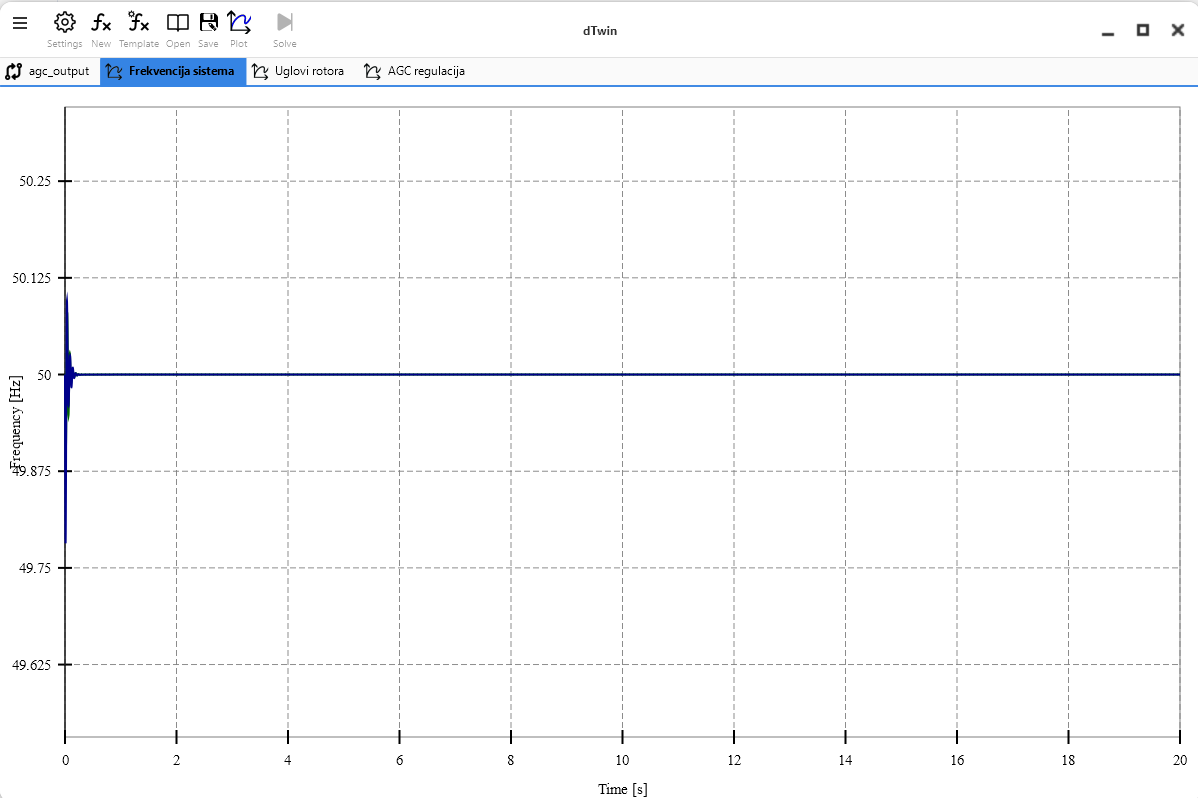
\includegraphics[width=0.8\textwidth]{case9frek.png}
    \caption{IEEE Case 9 -- frekvencija sistema: propad nakon skoka opterećenja
  i povratak na 50~Hz djelovanjem AGC regulacije}
    \label{fig:moj_izbor_oznake}
\end{figure}


 \begin{figure}[H]
    \centering
    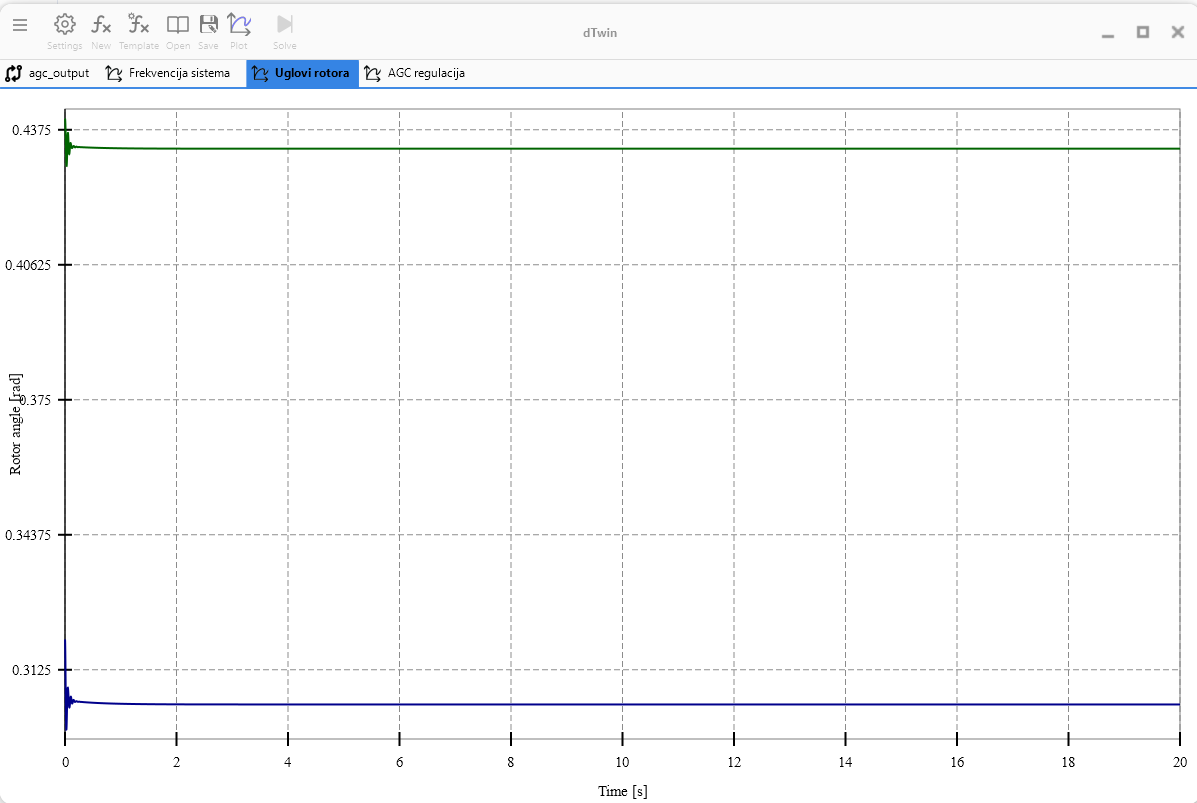
\includegraphics[width=0.8\textwidth]{case9uglovi.png}
        \caption{IEEE Case 9 -- uglovi rotora generatora 2 i 3}
    \label{fig:moj_izbor_oznake}
\end{figure}

\begin{figure}[H]
    \centering
    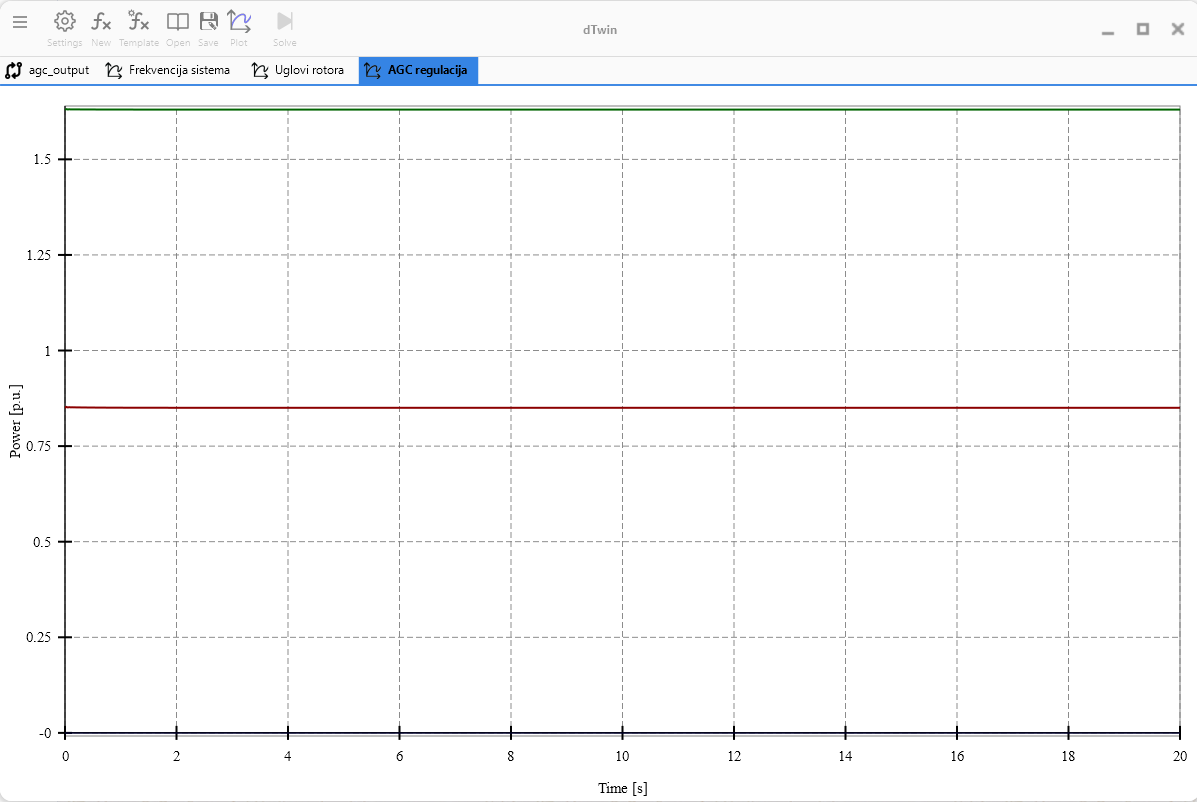
\includegraphics[width=0.8\textwidth]{case9reg.png}
     \caption{IEEE Case 9 -- mehanička snaga i integrator sekundarne regulacije}
    \label{fig:moj_izbor_oznake}
\end{figure}
 
 
\subsection{IEEE Case 30}
 
IEEE Case~30 (30 sabirnica, 41 grana) sadrži pet PV generatora na sabirnicama
2, 13, 22, 23 i~27. U testiranoj konfiguraciji generatori 2 i~22 imaju AGC
regulaciju, dok su 13, 23 i~27 standardni -- čime je direktno demonstrirana
specifikacija teme: \emph{navođenje generatora traženog tipa po broju, dok
ostali generatori dobijaju standardni model}. Generisani model sadrži
\textbf{14 diferencijalnih} i \textbf{60 algebarskih jednačina}. Sistem je
stabilan tokom cijele simulacije; AGC generatori preuzimaju kompenzaciju
poremećaja i vraćaju frekvenciju na nominalnu vrijednost.

 \begin{figure}[H]
    \centering
    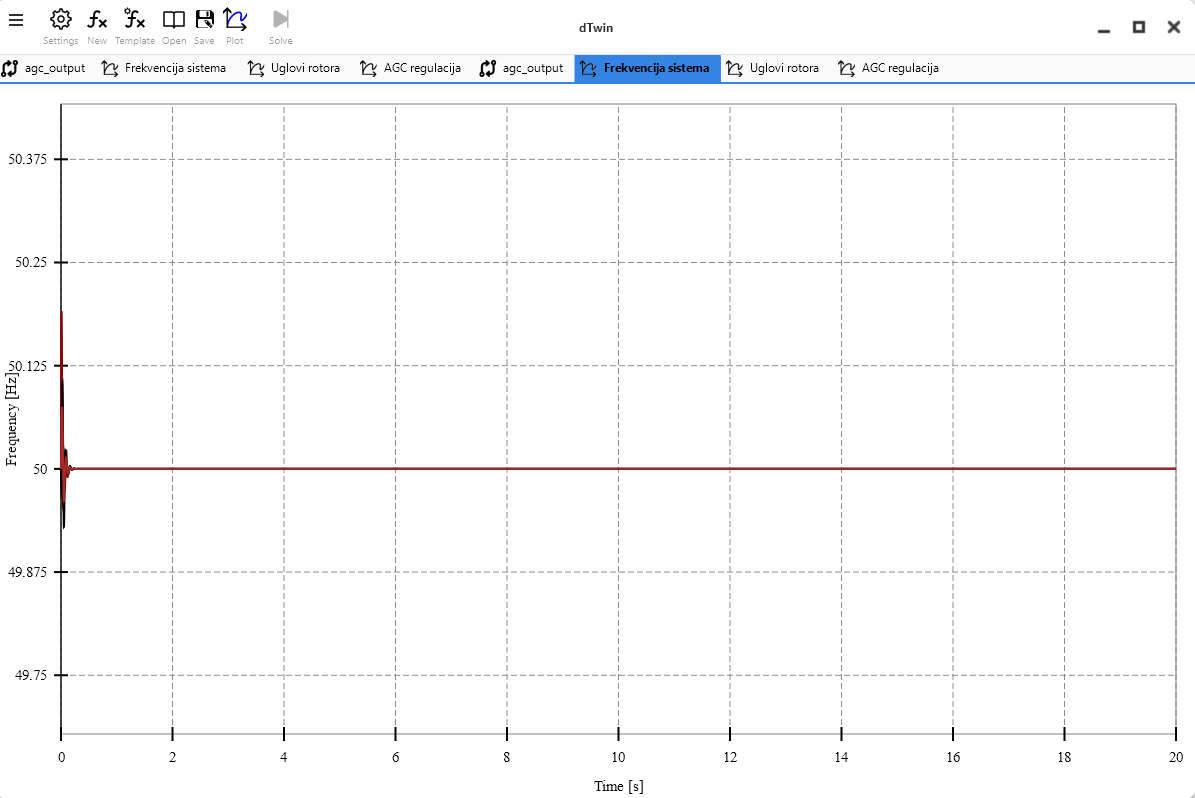
\includegraphics[width=0.8\textwidth]{case30frek.png}
          \caption{IEEE Case 30 -- frekvencija sistema}
    \label{fig:moj_izbor_oznake}
\end{figure}


 \begin{figure}[H]
    \centering
    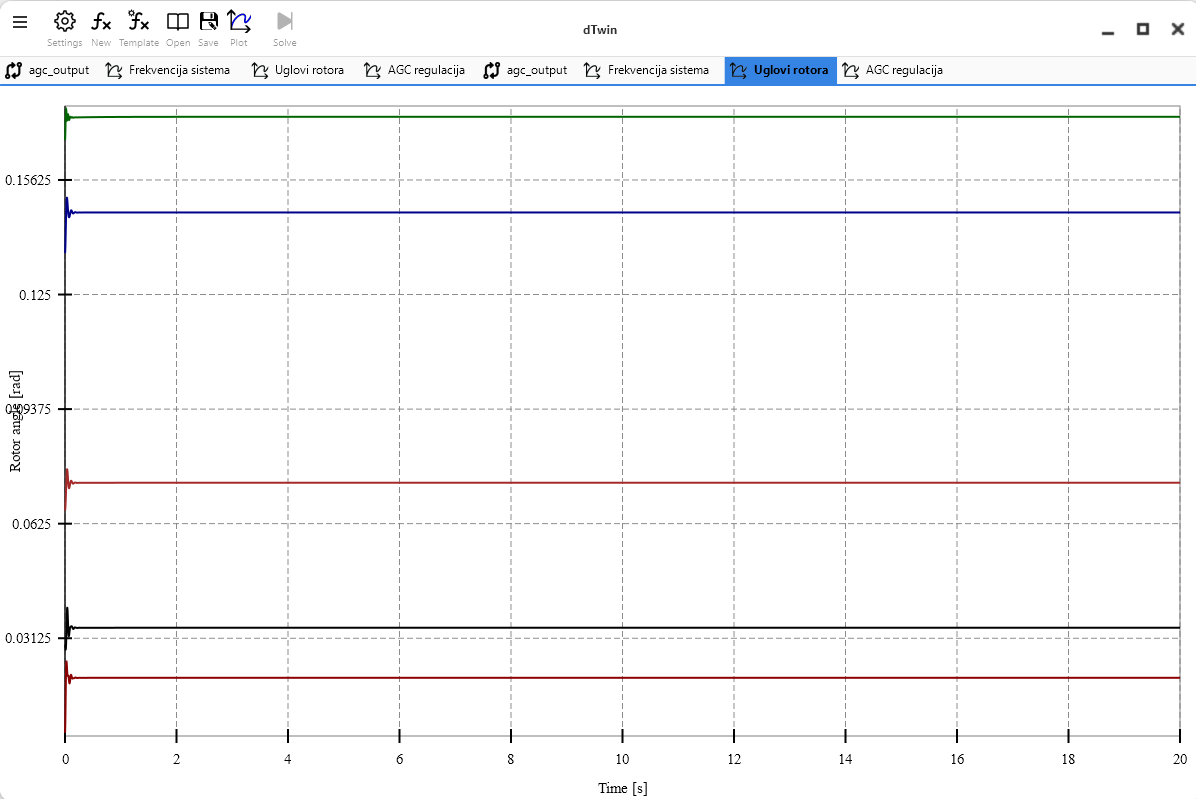
\includegraphics[width=0.8\textwidth]{case30uglovi.png}
     \caption{IEEE Case 30 -- uglovi rotora svih pet generatora (2 AGC + 3 standardna)}
    \label{fig:moj_izbor_oznake}
\end{figure}

\begin{figure}[H]
    \centering
    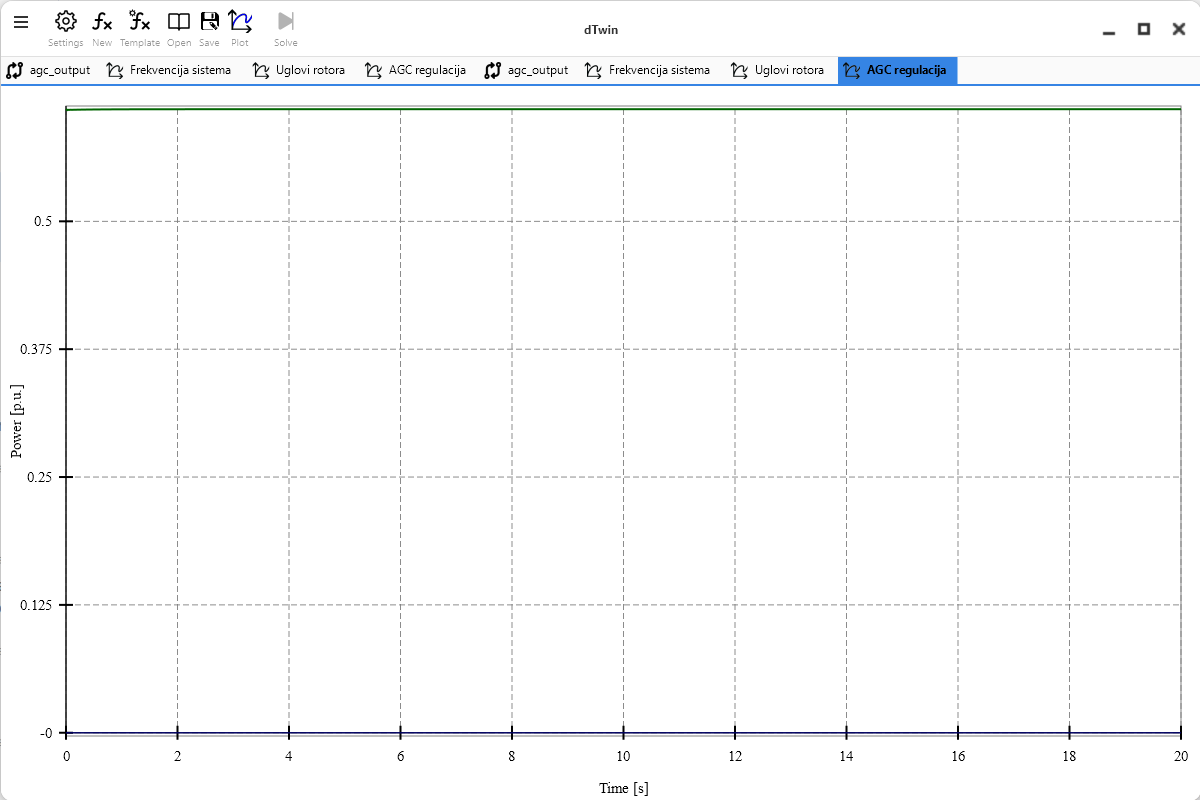
\includegraphics[width=0.8\textwidth]{case30reegulacija.png}
    \caption{IEEE Case 30 -- mehanička snaga i integrator sekundarne regulacije}
    \label{fig:moj_izbor_oznake}
\end{figure}
 
\subsection{IEEE Case 118}
 
IEEE Case~118 (118 sabirnica, 186 grana, 18 generatora sa aktivnom
proizvodnjom; referentna sabirnica je 69) testiran je sa AGC regulacijom na
generatorima 10 i~12. Generisani model sadrži \textbf{40 diferencijalnih} i
\textbf{236 algebarskih jednačina}. Uočava se da je za isti relativni
poremećaj propad frekvencije znatno manji nego kod malih mreža (oko
0{,}13~Hz) -- veći sistem posjeduje veću ekvivalentnu inerciju i krutost, što
je u skladu s teorijom. AGC vraća frekvenciju na nominalnu vrijednost za
manje od pola sekunde.

 \begin{figure}[H]
    \centering
    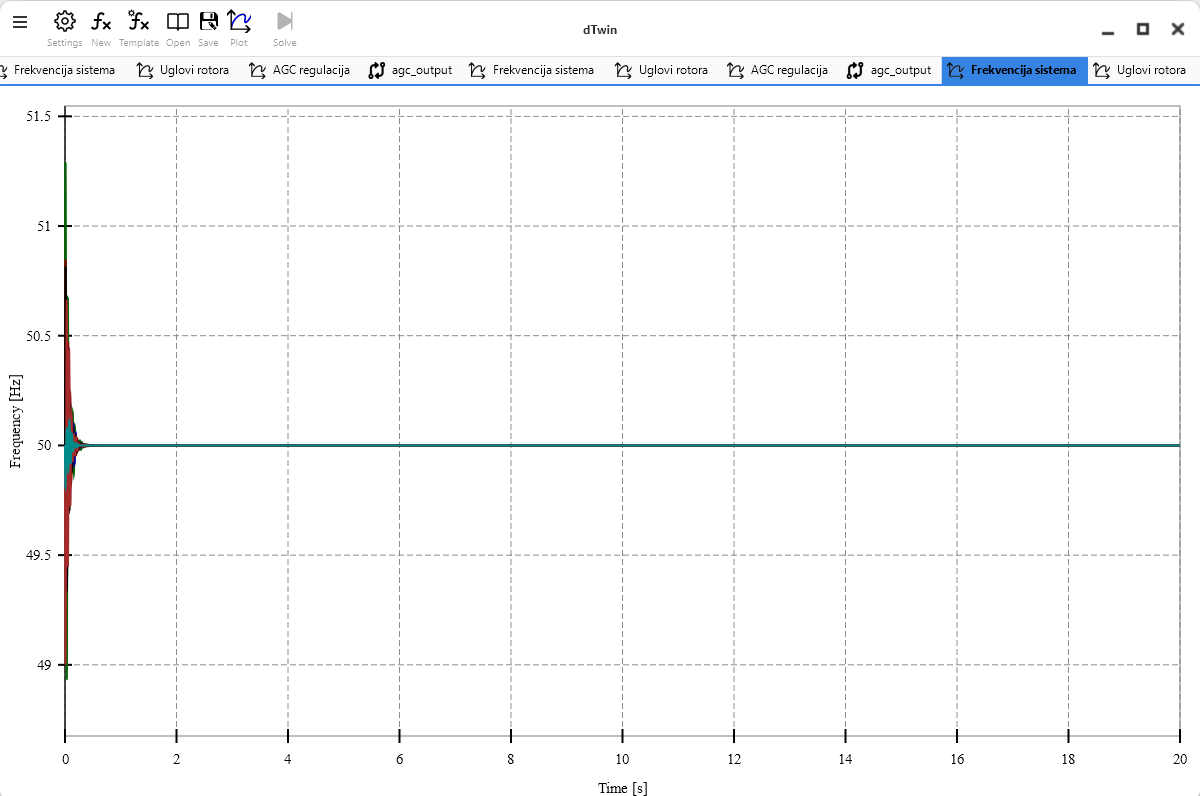
\includegraphics[width=0.8\textwidth]{case118frek.png}
    \caption{IEEE Case 118 -- frekvencija sistema: mali propad i brza
  regulacija karakteristični za velike sisteme}
    \label{fig:moj_izbor_oznake}
\end{figure}

\begin{figure}[H]
    \centering
    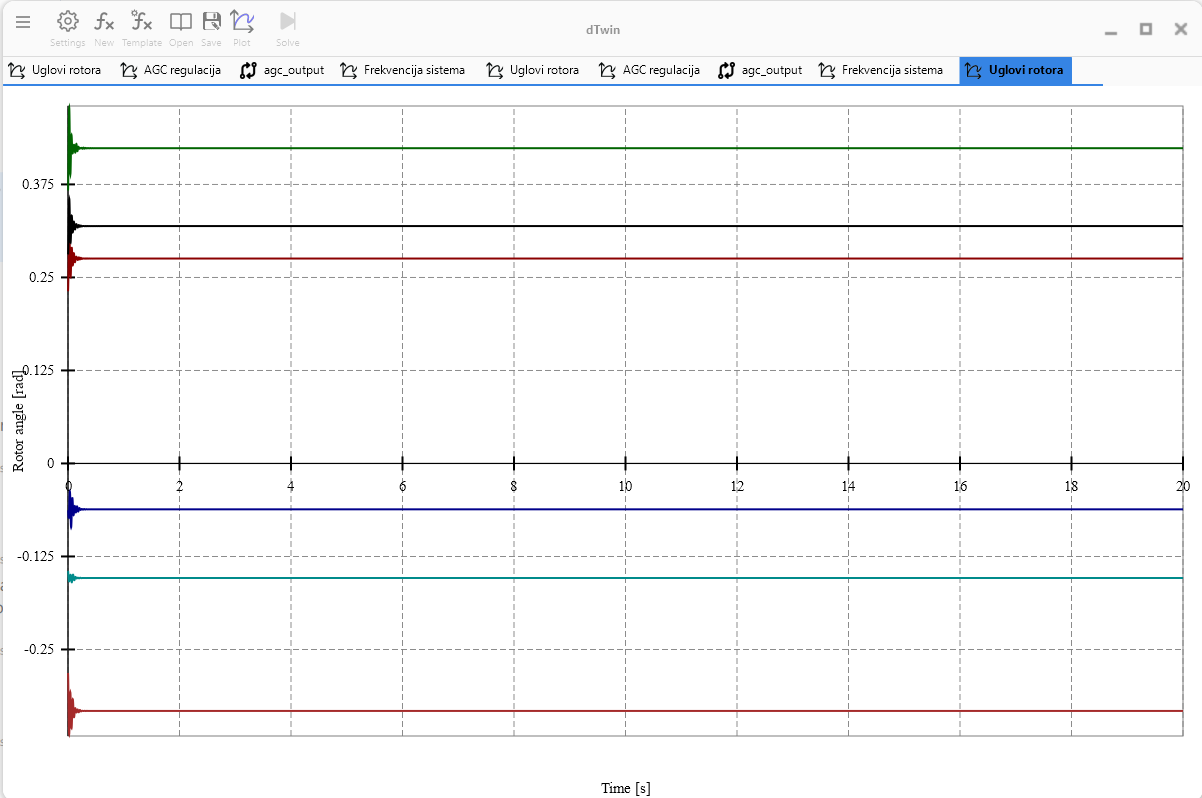
\includegraphics[width=0.8\textwidth]{case118uglovi.png}
     \caption{IEEE Case 118 -- uglovi rotora (prikazano 6 generatora)}
    \label{fig:moj_izbor_oznake}
\end{figure}

 
\subsection{IEEE Case 300 -- diskusija ograničenja}
 
Konverzija \texttt{case300} mreže (300 sabirnica, 411 grana, 56 generatora)
uspješno se izvršava i generiše strukturno ispravan model sa
\textbf{116 diferencijalnih} i \textbf{600 algebarskih jednačina}. Vremenska
simulacija, međutim, otkriva granicu primjenjivosti klasičnog modela
generatora: stvarna \texttt{case300} mreža ima izrazito neujednačen naponski
profil (naponi od 0{,}80 do 1{,}09~p.u.), zbog čega pojedine mašine iz tokova
snaga izlaze u podpobuđenom režimu rada, na samoj granici statičke
stabilnosti, te tokom simulacije gube sinhronizam. Vjerno modelovanje ovakvih
radnih tačaka zahtijeva detaljnije modele generatora sa regulatorima pobude
(AVR) i pripadajućim limiterima, što prevazilazi okvir teme. Konvertor pri
tome u potpunosti obavlja svoju funkciju -- generisani model je strukturno i
numerički ispravan, a ograničenje je svojstvo klasičnog modela, ne
implementacije.
\begin{figure}[H]
    \centering
    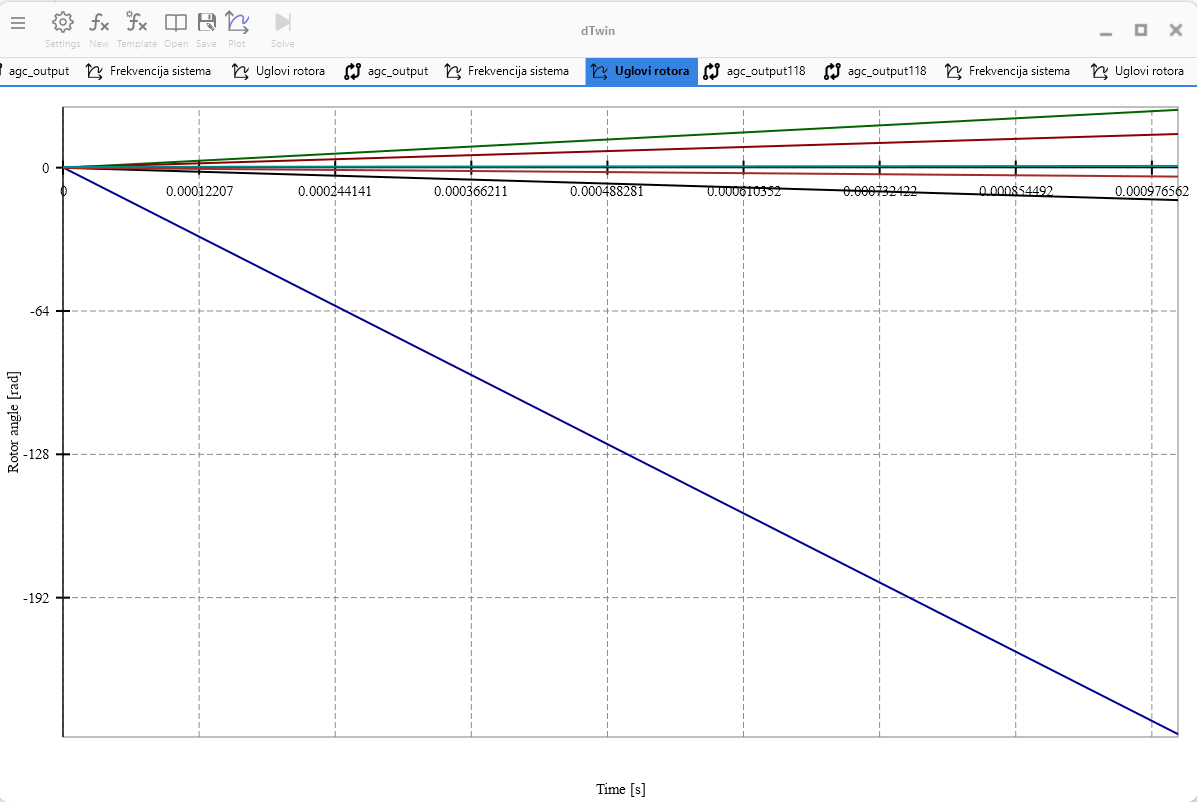
\includegraphics[width=0.8\textwidth]{case300.png}
     \caption{IEEE Case 300 -- uglovi rotora }
    \label{fig:moj_izbor_oznake}
\end{figure}
 
\subsection{Diskusija rezultata}
 
Ključni doprinos numeričkoj robusnosti rješenja je inicijalizacijski podmodel
sa tokovima snaga: dinamička simulacija kreće iz tačne ravnotežne tačke, pa
je jedini poremećaj onaj namjerno zadan (skok opterećenja). Bez ove
inicijalizacije neuravnoteženi početni uslovi generišu velike debalanse snage
u $t=0$ i vode u numeričku divergenciju već u prvim milisekundama simulacije.
Rezultati na sva tri uspješno simulirana sistema pokazuju identičan
kvalitativan obrazac -- propad frekvencije, prigušene oscilacije, povratak na
tačno 50~Hz -- uz kvantitativne razlike (dubina propada, brzina odziva)
konzistentne sa veličinom sistema.

 \newpage
% ============ 5. ZAKLJUČAK ============
\section{Zaključak}
 
U okviru projekta razvijen je dinamički konvertor koji statičke MATPOWER
podatke elektroenergetske mreže automatski pretvara u dinamičke modele sa AGC
regulacijom frekvencije, u obliku natID plugina (dll) sa grafičkim
interfejsom, XML konfiguracijom generatora, višenitnom konverzijom sa
indikatorom napretka i korištenjem natID dense matrica za admitansnu matricu
mreže. Uspješna sekundarna regulacija frekvencije demonstrirana je na
testnim sistemima Case~9, Case~30 i Case~118: nakon skoka opterećenja
frekvencija se u svim slučajevima vraća tačno na nominalnih 50~Hz, čime je
potvrđena ispravnost implementiranog AGC modela. Za Case~300 konverzija je
uspješna, a simulacija je identifikovana kao ograničenje klasičnog modela
generatora u mrežama sa ekstremnim naponskim profilom. Arhitektura konvertora
je generička -- svi algoritmi (parsiranje, Ybus, generisanje jednačina,
inicijalizacija) rade nad proizvoljnom mrežom, bez posebnih slučajeva po
testnom sistemu.
 
% ============ LITERATURA ============
\begin{thebibliography}{9}
\bibitem{kundur} P.~Kundur, \emph{Power System Stability and Control},
McGraw-Hill, 1994.
\bibitem{matpower} R.~D.~Zimmerman, C.~E.~Murillo-S\'anchez,
\emph{MATPOWER}, \url{https://github.com/MATPOWER/matpower}
\bibitem{natid} I.~Džafić, \emph{natID biblioteka},
\url{https://github.com/idzafic/natID}
\bibitem{dtwin} I.~Džafić, \emph{dTwin -- Components for digital twinning},
\url{https://github.com/idzafic/dTwin}
\end{thebibliography}
 
\end{document}
